\documentclass[10pt,a4paper]{article}
\usepackage{times}
\usepackage{latexsym}
\setlength{\parskip}{0.5\baselineskip}
\usepackage{indentfirst}
\usepackage{graphicx}
\graphicspath{{./}}

\title{Results Analysis}
\date{\vspace{-5ex}}
\begin{document}
\maketitle
%Which parameter setting "fits" the observed cascade (from file cascade.txt) best? Why? How can you measure the goodness of fit? What is a possible explanation of the observed behavior of bad fits? How can you further improve the fit?

The "Heterogeneous" parameter setting "fits" the observed cascade best. Firstly, we can see this intuitively in Figure 1. It's curve fits the observed cascade's best than others. Secondly, the most tight confidence intervals of it suggests it's a best parameter. What's more, the goodness of fit also indicates it fits best.

\begin{figure}[h]
    \centering
    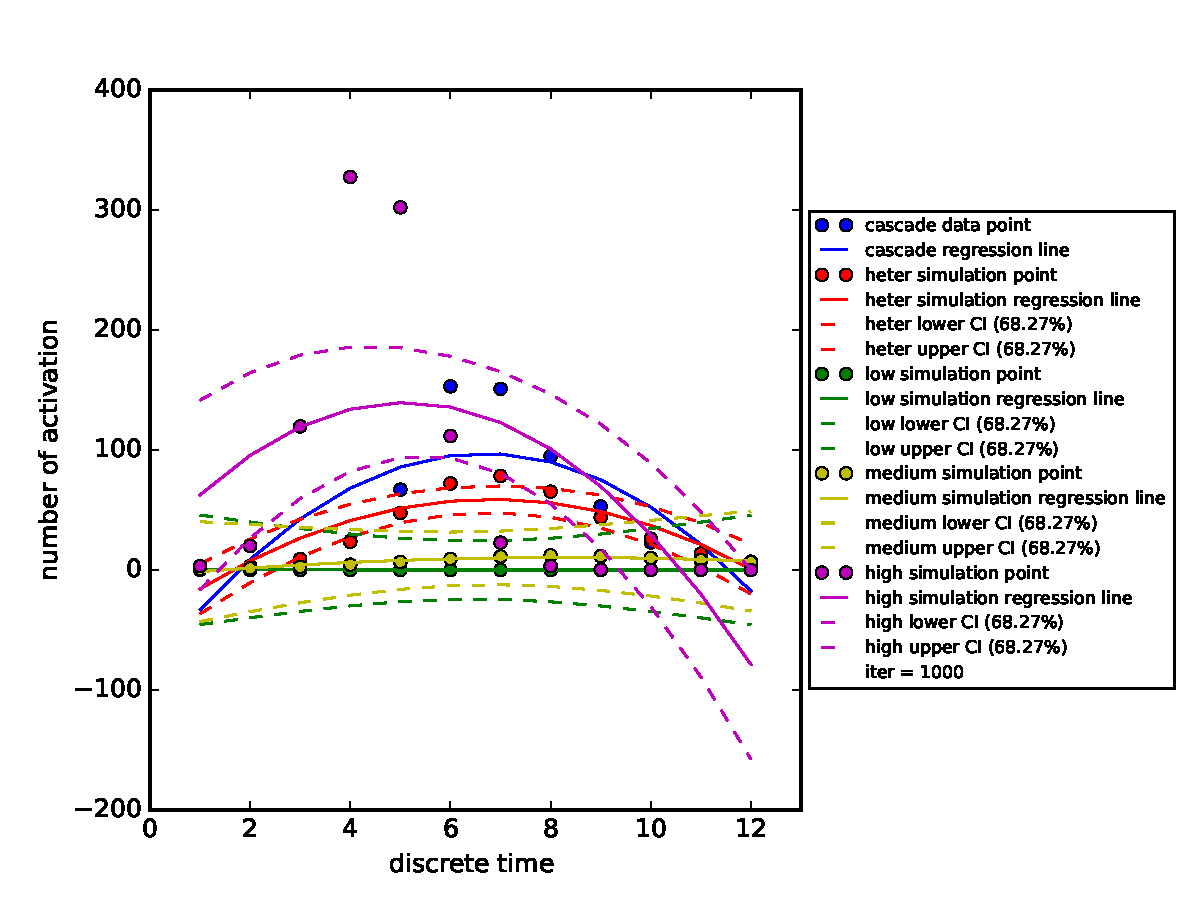
\includegraphics[width=0.7\textwidth, height=0.3\textheight]{simulate}
    \caption{The Simulation Results}
    \label{fig:simulate}
\end{figure}

We adopt Mean Square Error(MSE) to measure the goodness of fit. As we know, the coefficient of determination(denoted \(R^2\)) is an inadequate measure for the goodness of fit in nonlinear models. The MSE is an absolute fit other than a relative measure, like \(R^2\). Lower values of MSE indicate better fit. It's formula is:
\begin{equation}
    MSE=\frac{1}{n}\sum_{i=1}^{n}(\hat{Y}_{i}-Y_{i})^{2}
\end{equation}
where \(\hat{Y}\) is a vector of \(n\) predictions, and \(Y\) is the vector of observed values. 

In these simulations, the MSE of model with "Heterogeneous", "Low", "Middle" and "High" parameter setting are about \(1104.3\), \(5312.7\), \(4866.4\) and \(10777.6\) respectively. So the "Heterogeneous" parameter setting "fits" the observered cascade best of all the four.

For the "Low" parameter setting, we can see its curve is nearly a horizontal line. This is because the probability \(0.01\) is too small. The propagation process would be stopped easily at the start period. As the figure 1 shows, there is almost none of nodes are actived under this setting. This is the same reason for "Middle" parameter setting. Though the \(0.05\) is a little higher than \(0.01\). 

While, for the "High" parameter setting, most of the nodes in graph would be actived at the start, so it will stop soon with no inactive nodes found in each iteration. Figure 1 shows it actives aroud 300 nodes at time \(4\) and \(5\) respectively. It "consumed" the inactive nodes quickly. 

In fact, the "Heterogeneous" parameter setting does not fit the observed cascade so perfect. It also suffer the same problem as the "Low" and "Middle" parameter setting. In the \(1000\) simulations, some iterations are discontinued with no active nodes found before time \(12\). This makes the average of total number of activations in this simulation is obviously less than the observed cascade's. 

In order to sovle this problem, we should take another key parameter, \(p_{e}(u)\)(the probalility that an inactive node spontaneously activates due to external factors), into account. This factor can add extra active nodes to increase the average of total number of activations. But for avoiding the trouble of "High" parameter setting, this value doesn't be too large. In my view, it should be obtained by many experiements. 

%For example, there are 16 nodes as the out-neighbours of the starting node 448 at t=1, but only 14.85\% to active node at t=2.

\end{document}
